\documentclass[11pt,a4paper]{article}
\usepackage[utf8]{inputenc}
\usepackage[T1]{fontenc}
\usepackage[margin=2.5cm]{geometry}
\usepackage{amsmath,amssymb}
\usepackage{graphicx}
\usepackage{booktabs}
\usepackage{float}
\usepackage{siunitx}
\usepackage{microtype}
\usepackage{xcolor}
\usepackage[font=small,labelfont=bf]{caption}
\usepackage[authoryear,round]{natbib}
\usepackage[colorlinks=true,linkcolor=blue!50!black,citecolor=blue!50!black,urlcolor=blue!50!black]{hyperref}
\usepackage[capitalise,noabbrev]{cleveref}

\graphicspath{{../figures/}}
\newcommand{\chem}[1]{\ensuremath{\mathrm{#1}}}

\title{Ore Geochemistry from Hyperspectral Images:\\ an Honest Baseline on HIDSAG}
\author{Juan Carlos Chavarr\'ia Morales\\[2pt]
  \small M.Sc.\ Optimization, Hochschule Bielefeld (HSBI)\\
  \small Course project, \emph{Machine Vision}}
\date{October 2026}

\begin{document}
\maketitle

\begin{abstract}
The feed of a semi-autogenous grinding (SAG) mill is characterised by sampling batches of ore and analysing them in
the laboratory; hyperspectral imaging of such samples could estimate their composition faster and at lower cost than
chemical assays. We test this idea on the public HIDSAG GEOCHEM data set \citep{Ehrenfeld2023}:
28 samples of porphyry copper ore, imaged in the visible to short-wave infrared (\SIrange{400}{2500}{nm}) and assayed
for 18 elements by portable X-ray fluorescence. Because every image of a sample carries the same label, the only
honest test is on samples the model has never seen. Under this test, a principal-component ridge regression on the
mean spectrum of each image reduces the error of the trivial mean predictor by \SI{29}{\percent} on average over the
nine major elements, and by about half for Ca and Fe; a 1D convolutional network does worse than this linear model.
The camera sees minerals, not elements: Al and K follow the Al--OH absorption of muscovite, Ca the molecular-water
band, and Cu is predicted through its association with alteration minerals. Grain size changes the absorption
depths more than composition does. The near-perfect accuracy published for this data set cannot be reproduced with
any split of the data that we tried. Code and data: \citet{Repo}.
\end{abstract}

% =====================================================================================================================
\section{Motivation}

The throughput and the energy consumption of a SAG mill depend on properties of its feed such as hardness, moisture
and clay content. These properties are not observed continuously: batches of ore are sampled, and each sample is
characterised by a set of estimation techniques, from chemical assays to metallurgical tests. Geometallurgy links
the results to the mineralogy and the chemistry of the ore. Among these techniques, reflectance spectroscopy is fast,
non-destructive and cheap per sample; if it can estimate the chemistry of a sampled batch, it can complement or
partly replace slower assays, and its estimates can serve as inputs to models of the mill. This report is the first
step of that chain: \emph{how well can hyperspectral
images predict the chemical composition of an ore sample?} The second step, from composition and spectra to the
variables of the mill, is outside its scope; it is discussed briefly in \cref{sec:next}.

The project was done for a course on machine vision with a free choice of topic. Its first version, a Jupyter
notebook, trained a convolutional network on 28 mean spectra and evaluated it on a random split. This report is a
re-analysis that asks three questions the notebook did not ask:
\begin{enumerate}
  \item What is an honest estimate of the prediction error, and is it better than chance?
  \item What does the camera physically see, and what in the images is not ore?
  \item Why are the accuracies published for this data set so much better?
\end{enumerate}

% =====================================================================================================================
\section{Materials}\label{sec:data}

HIDSAG \citep{Ehrenfeld2023,HIDSAGdata} contains five subsets of geometallurgical samples from Chilean copper
deposits, each imaged with two push-broom cameras: a VNIR camera (942 bands, \SIrange{400}{1000}{nm}) and a SWIR
camera (268 bands, \SIrange{1000}{2500}{nm}), co-registered at the resolution of the SWIR camera. We use the subset
GEOCHEM: 28 crushed samples of SAG feed, each split into a fine and a coarse size fraction and photographed in
two crops per fraction, 106 crops of about $70 \times 150$ pixels in total. Each sample has one pXRF analysis of
18 elements. We study the nine elements whose variation across samples is clearly above the detection limit
(Al, Si, P, S, K, Ca, Ti, Fe, Cu); Zn, As, Pb, Mo and the other traces are reported in the repository.

\paragraph{The unit of independence is the sample.} The 106 crops and their \num{1.1e6} pixels share 28 labels.
The amount of information about the relation between spectrum and composition is therefore set by the 28
samples, not by the number of pixels. A model that is tested on a pixel, a patch or a crop of a sample that is also
in its training set can succeed by recognising the sample instead of predicting its composition
\citep{Roberts2017,Kaufman2012}.

\paragraph{Spectral features.} The raw counts are divided by $10^4$. The VNIR spectrum is averaged into \SI{10}{nm}
bins between 420 and \SI{1000}{nm} (58 features) to remove its noise; the SWIR spectrum is kept between 1000 and
\SI{2450}{nm} (259 features). Each crop is summarised by its mean spectrum (\emph{crop level}) or by 40 means of 25
random pixels (\emph{patch level}), drawn from 1000 pixels stored per crop by the extraction script.
\Cref{fig:spectra} shows the spectra of the samples with the lowest and the highest Ca content.

\begin{figure}[t]
  \centering
  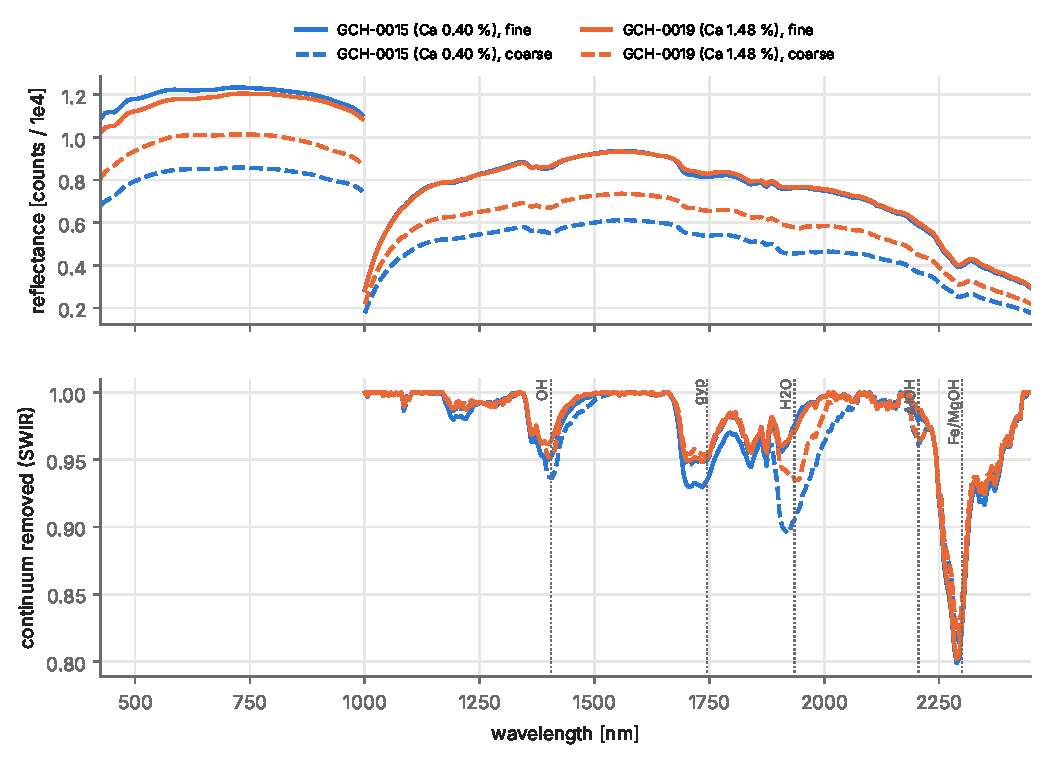
\includegraphics[width=0.92\linewidth]{spectra.pdf}
  \caption{Mean spectra of the samples with the lowest and the highest Ca content. Top: reflectance of the two
    cameras; coarse crops (dashed) are darker. Bottom: SWIR spectrum divided by its convex hull (continuum removal,
    \citealp{Clark1984}). The difference between the fine and the coarse fraction of the \emph{same} sample is
    larger than the difference between the two samples; in this pair the high-Ca sample even has the weaker water
    band, against the trend over all samples (\cref{tab:features}).}
  \label{fig:spectra}
\end{figure}

% =====================================================================================================================
\section{What the camera sees}\label{sec:physics}

Visible and short-wave infrared light does not interact with elements but with chemical bonds and electronic
transitions in minerals \citep{Hunt1977}: vibrations of \chem{OH} and \chem{H_2O} near 1400 and \SI{1900}{nm},
\chem{Al\text{-}OH} near \SI{2200}{nm} (muscovite, kaolinite), \chem{Fe/Mg\text{-}OH} near \SI{2300}{nm} (chlorite,
biotite), and charge transfer of ferric iron below \SI{550}{nm}. Elements can therefore be predicted only to the
extent that they reside in, or co-vary with, minerals that have such absorptions.

\Cref{fig:correlation} shows the correlation of the continuum-removed reflectance with each element across the 28
samples, and \cref{tab:features} the same for five absorption band depths. The clearest pattern is that of
muscovite (sericite alteration): Al and K go with a deeper Al--OH band at \SI{2205}{nm} and a deeper OH band at
\SI{1405}{nm}, and K with a shallower Fe/Mg--OH band ($r = -0.67$). Ca goes with a deeper molecular-water band at
\SI{1935}{nm} ($r = 0.49$), consistent with gypsum or hydrated clays, but only weakly with the sulfate band of gypsum
at \SI{1745}{nm}. Cu and Fe have no diagnostic absorption in this range; Cu-rich samples absorb more between 1700 and
\SI{1880}{nm} and at the OH band, i.e.\ copper is predicted through the alteration that accompanies the
mineralisation, not through copper minerals. With 28 samples, $|r| > 0.37$ is needed for significance at the
\SI{5}{\percent} level, and a few hundred bands are tested: single correlations are fragile, and the best single
band generalises poorly (\cref{sec:results}).

\begin{figure}[t]
  \centering
  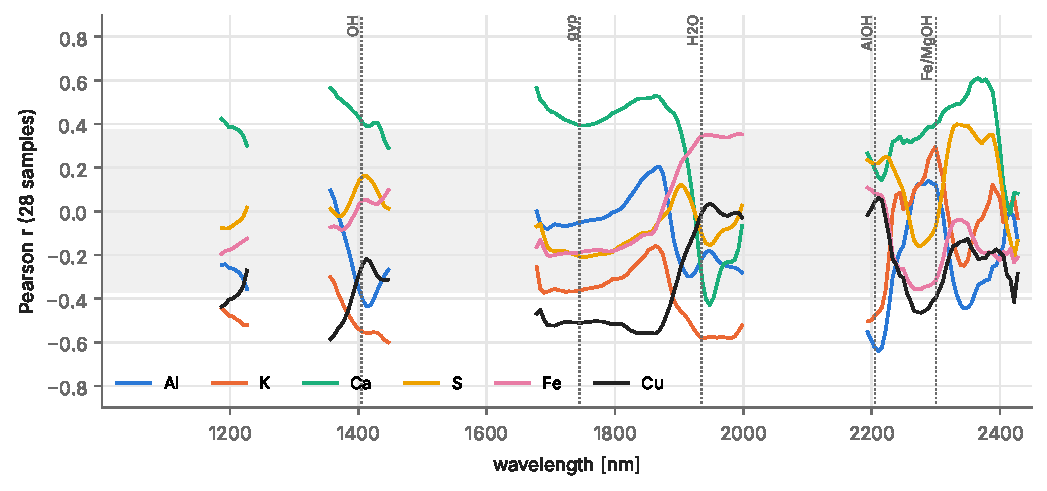
\includegraphics[width=0.92\linewidth]{correlation.pdf}
  \caption{Correlation between continuum-removed SWIR reflectance and composition over the 28 samples. Negative
    values mean a deeper absorption in samples richer in the element. Bands where no sample absorbs (continuum
    $\approx 1$) are omitted. Grey: $|r| < 0.37$, not significant at $p = 0.05$ for a single band.}
  \label{fig:correlation}
\end{figure}

\begin{table}[t]
  \centering\small
  \caption{Band depths \citep{Clark1984} of the main absorption features: correlation of the sample means with the
    composition, the spread between samples, and the mean difference between the coarse and the fine fraction of
    the same sample (25 samples with both fractions).}
  \label{tab:features}
  \resizebox{\linewidth}{!}{\begin{tabular}{lrrrrrrrr}
\toprule
& \multicolumn{6}{c}{correlation with element (28 samples)} & \multicolumn{2}{c}{variation} \\ \cmidrule(lr){2-7}\cmidrule(lr){8-9}
feature & Al & K & S & Ca & Fe & Cu & between samples (sd) & coarse $-$ fine \\
\midrule
OH 1405 & +0.43 & +0.55 & $-$0.16 & $-$0.39 & $-$0.04 & +0.22 & 0.0057 & +0.0123 \\
gyp 1745 & +0.08 & +0.38 & +0.38 & +0.21 & +0.09 & +0.27 & 0.0007 & +0.0004 \\
H2O 1935 & +0.25 & +0.56 & +0.13 & +0.49 & $-$0.35 & $-$0.13 & 0.0091 & +0.0316 \\
AlOH 2205 & +0.58 & +0.52 & $-$0.20 & $-$0.14 & $-$0.15 & $-$0.09 & 0.0062 & +0.0211 \\
Fe/MgOH 2300 & $-$0.40 & $-$0.67 & +0.31 & $-$0.11 & +0.29 & +0.23 & 0.0021 & $-$0.0016 \\
red/blue 700/480 & $-$0.20 & $-$0.02 & $-$0.16 & +0.39 & $-$0.27 & $-$0.32 & 0.0129 & +0.0222 \\
\bottomrule
\end{tabular}
}
\end{table}

\paragraph{Grain size dominates the absorption depths.} The last two columns of \cref{tab:features} carry the most
important result of this section. For the water band at \SI{1935}{nm} and the Al--OH band at \SI{2205}{nm}, the
coarse fraction of a sample absorbs more than its fine fraction by 3.5 times the standard deviation between samples,
consistently in all 25 pairs. This is the expected physics (longer optical paths in larger grains), but it means that
a feature extracted from an image depends more on the particle size distribution than on the composition. Unless the
sample preparation fixes the size fraction, this effect has to be modelled or measured.

\paragraph{Not every pixel is ore.} \Cref{fig:maps} maps the band depths pixel by pixel for two samples and clusters
the continuum-removed SWIR spectra of all pixels with $k$-means. One cluster has absorptions at 1210, 1730 and
\SI{2310}{nm}: the C--H overtones of plastic, i.e.\ the sample tray, visible at the edges of the crops. Over all 106
crops, the tray makes up a median of \SI{4}{\percent} and at most \SI{17}{\percent} of the pixels. The other clusters
separate the size fractions and follow vertical stripes of the push-broom sensor rather than individual particles:
at the resolution of these cubes, the fine fraction cannot be resolved into single grains.

\begin{figure}[p]
  \centering
  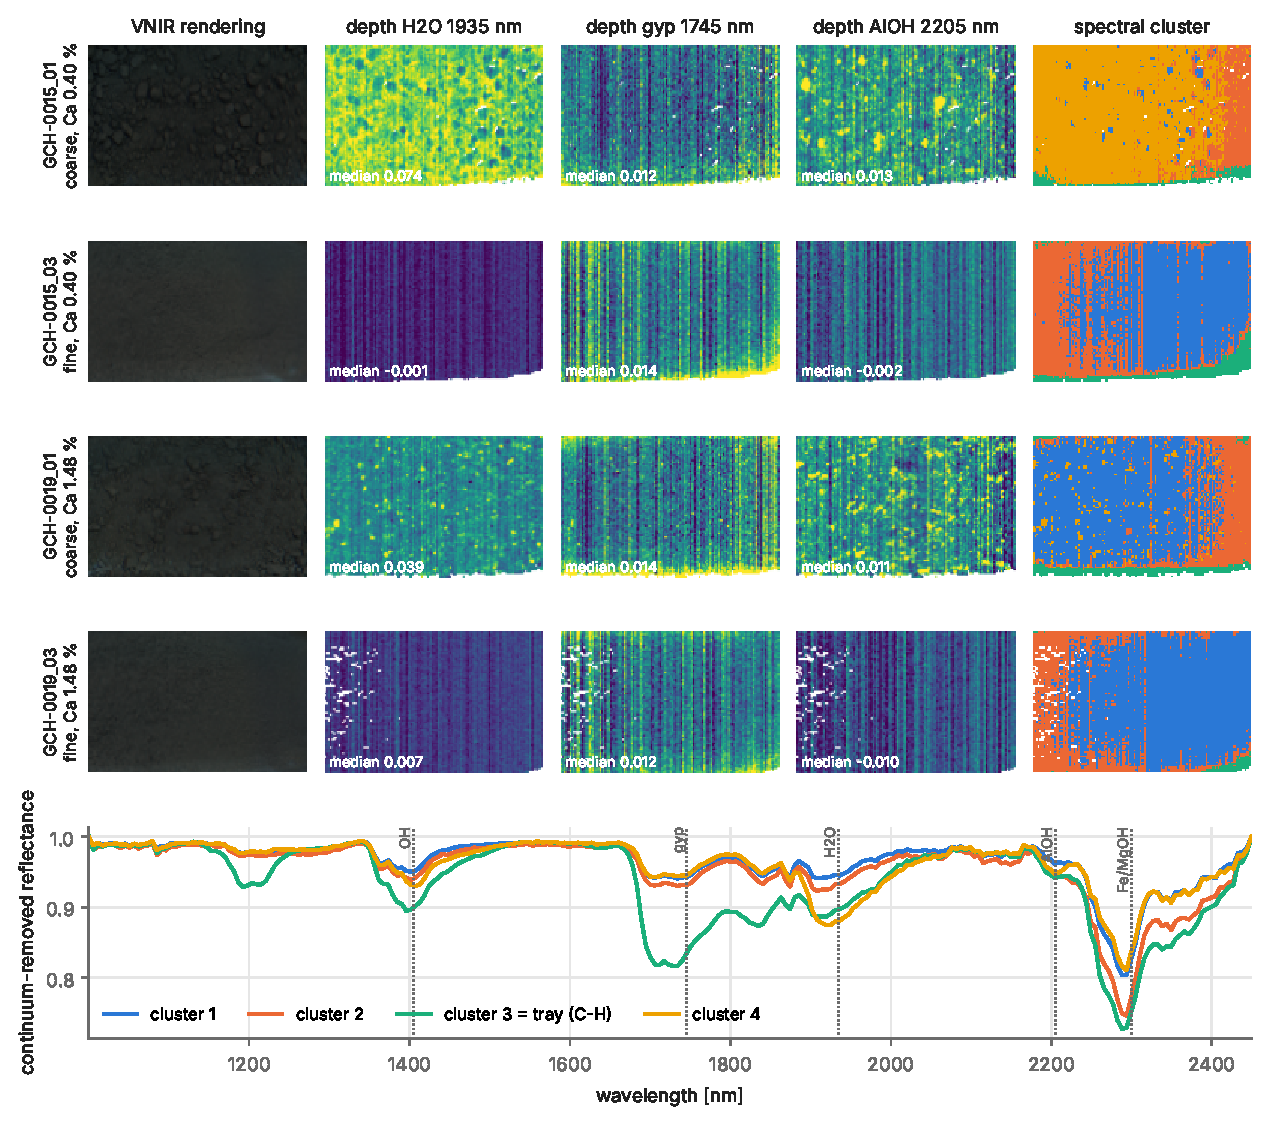
\includegraphics[width=\linewidth]{mineral_maps.pdf}
  \caption{Pixel maps of a low-Ca (GCH-0015) and a high-Ca (GCH-0019) sample, coarse (01) and fine (03) crops.
    Columns: VNIR rendering, band depths at 1935, 1745 and \SI{2205}{nm} (same colour scale per column), and
    $k$-means clusters of the continuum-removed SWIR spectra, with the cluster centres below. The tray cluster
    appears at the lower edge of the crops. The maps differ more between the two crops of one sample than between
    the two samples.}
  \label{fig:maps}
\end{figure}

% =====================================================================================================================
\section{Method}\label{sec:method}

\paragraph{Validation.} All results are \emph{leave-one-sample-out} (LOSO): each sample is predicted by a model
trained on the other 27, and every hyper-parameter is chosen by an inner cross-validation grouped by sample on the
training samples only. The predictions for the crops or patches of a test sample are averaged into one prediction
per sample. The reference is the mean predictor, which predicts the mean composition of the training samples. We
report the skill
\[
  \text{skill} = 1 - \frac{\text{MAE}}{\text{MAE}_{\text{mean predictor}}},
\]
the fraction of the error of the mean predictor that the model removes (0: no better than the mean, 1: perfect),
and the predictive $Q^2$, the analogous ratio of squared errors. The mean absolute percentage error (MAPE) is given
for comparison with the literature, but it depends on the level of the element and says nothing without the
reference of the mean predictor. Whether a skill is better than chance is tested by permuting the labels between
whole samples and repeating the complete LOSO procedure 100 times \citep{Ojala2010}.

\paragraph{Models.} Partial least squares (PLS, \citealp{Wold2001}), the standard of chemometrics; principal
component analysis followed by ridge regression (PCA + ridge); a re-implementation of the HIDSAG validation pipeline
\citep{Egana2020}, $k$-means clustering of patch spectra with one PLS per cluster; a small 1D convolutional network
(three convolution layers, about \num{4000} weights, early stopping on held-out samples); and, as the most
interpretable competitor, a single best band per element, re-selected in every fold. All models predict the 18
standardised elements jointly. Pre-processing \citep{Rinnan2009}: none (raw), standard normal variate (SNV), or SNV
followed by a Savitzky--Golay first derivative, computed separately for each camera.

% =====================================================================================================================
\section{Results}\label{sec:results}

\Cref{tab:benchmark,fig:skill} summarise the benchmark. The best model, PCA + ridge on the raw crop means, removes
\SI{29}{\percent} of the error of the mean predictor on average. The elements fall into three groups:
\begin{itemize}
  \item \textbf{Ca and Fe} (skill 0.50 and 0.49, $Q^2$ 0.71 and 0.69): predictable; Ca through the water band,
    Fe through information spread over the whole spectrum rather than a single feature;
  \item \textbf{K, S, Al, Cu} (0.28--0.33): partly predictable, through muscovite (Al, K) and through the
    association of sulfides with alteration (S, Cu; S, Fe and Cu correlate with each other at $r \approx 0.55$);
  \item \textbf{Si, P, Ti} (0.11--0.16): hardly predictable; quartz, apatite and rutile have no absorptions in this
    range.
\end{itemize}
The permutation test (\cref{tab:permutation}) confirms that the skill is not an artefact of the small sample: for
PCA + ridge, no permutation of the labels reaches the observed skill for eight of the nine elements ($p < 0.01$),
and for Si $p = 0.02$. Even the small skills of Si, P and Ti are real, if of little practical use. The predictions (\cref{fig:pred}) are shrunk towards the mean, as expected from a regularised
model trained on 27 points; the ranking of the samples is better than the absolute values.

\begin{table}[t]
  \centering\small
  \caption{Leave-one-sample-out benchmark: mean skill and $Q^2$ over the nine major elements, and skill per element.
    Patch level: 40 patches of 25 pixels per crop (4240 rows, still 28 samples).}
  \label{tab:benchmark}
  \resizebox{\linewidth}{!}{\begin{tabular}{lllrrrrrrrr}
\toprule
model & level & pre-proc. & skill & $Q^2$ & Al & K & S & Ca & Fe & Cu \\
\midrule
mean & crop & raw & +0.00 & $-$0.00 & $-$0.01 & +0.02 & $-$0.00 & $-$0.00 & $-$0.00 & $-$0.00 \\
best band & crop & SNV + 1st deriv. & +0.07 & +0.06 & +0.16 & +0.07 & $-$0.24 & +0.41 & +0.20 & +0.37 \\
PLS & crop & raw & +0.20 & +0.37 & +0.18 & +0.13 & +0.20 & +0.40 & +0.47 & +0.20 \\
PLS & crop & SNV + 1st deriv. & +0.24 & +0.40 & +0.25 & +0.03 & +0.27 & +0.48 & +0.39 & +0.30 \\
PCA + ridge & crop & raw & \textbf{+0.29} & +0.48 & +0.29 & +0.33 & +0.31 & +0.50 & +0.49 & +0.28 \\
PCA + ridge & crop & SNV + 1st deriv. & +0.27 & +0.46 & +0.22 & +0.26 & +0.31 & +0.50 & +0.38 & +0.30 \\
1D-CNN & crop & SNV & +0.02 & +0.04 & +0.07 & +0.03 & $-$0.01 & $-$0.02 & +0.12 & +0.02 \\
\midrule
PLS & patch & SNV & +0.26 & +0.44 & +0.23 & +0.26 & +0.31 & +0.52 & +0.32 & +0.26 \\
PCA + ridge & patch & SNV & +0.23 & +0.39 & +0.20 & +0.10 & +0.30 & +0.49 & +0.29 & +0.25 \\
cluster + PLS (HIDSAG-like) & patch & SNV & +0.22 & +0.39 & +0.14 & +0.23 & +0.38 & +0.41 & +0.27 & +0.31 \\
1D-CNN & patch & SNV & +0.17 & +0.32 & +0.14 & +0.22 & +0.10 & +0.31 & +0.21 & +0.17 \\
\bottomrule
\end{tabular}
}
\end{table}

\begin{figure}[t]
  \centering
  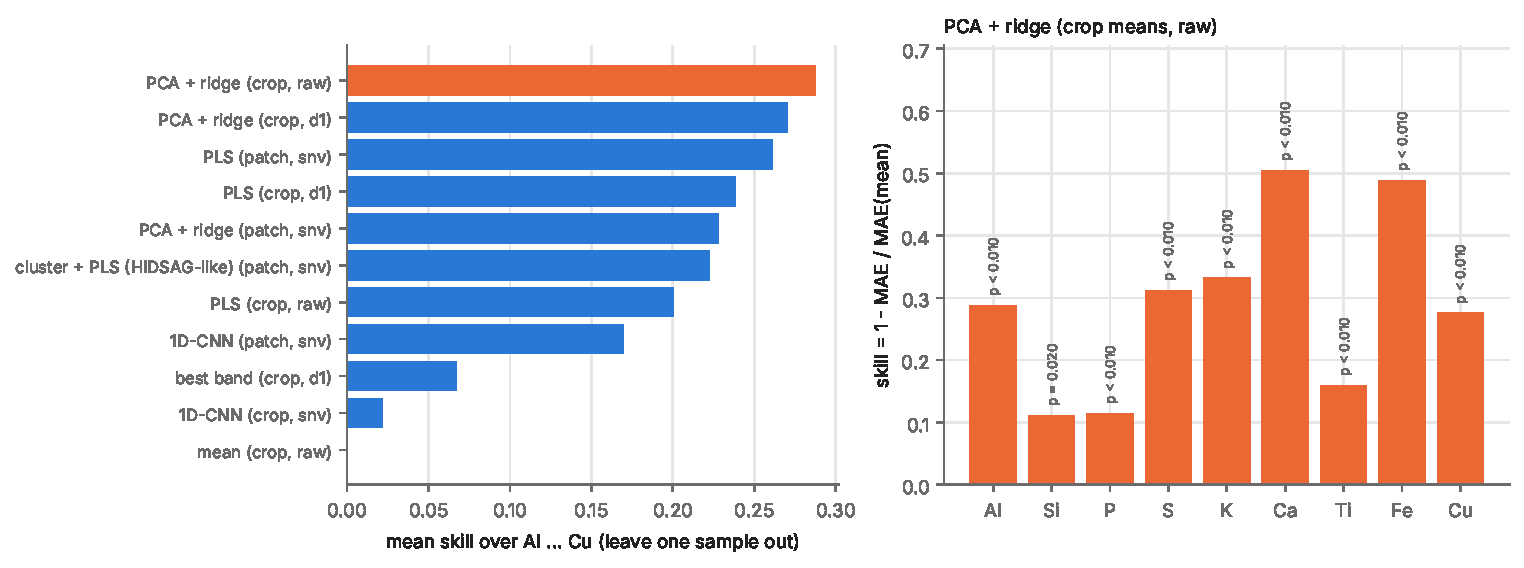
\includegraphics[width=\linewidth]{skill.pdf}
  \caption{Left: mean skill of all configurations (Al \ldots Cu). Right: skill of the best model per element, with
    the $p$-value of the permutation test (100 permutations of the labels between samples).}
  \label{fig:skill}
\end{figure}

\begin{table}[t]
  \centering\small
  \caption{Permutation test: LOSO skill and its $p$-value under 100 random re-assignments of the compositions to the
    samples (crop level).}
  \label{tab:permutation}
  \resizebox{\linewidth}{!}{\begin{tabular}{llrrrrrrrrr}
\toprule
model & & Al & Si & P & S & K & Ca & Ti & Fe & Cu \\
\midrule
PCA + ridge (raw) & skill & +0.29 & +0.11 & +0.11 & +0.31 & +0.33 & +0.50 & +0.16 & +0.49 & +0.28 \\
 & $p$ & $<$0.01 & 0.020 & $<$0.01 & $<$0.01 & $<$0.01 & $<$0.01 & $<$0.01 & $<$0.01 & $<$0.01 \\
PLS (SNV + 1st deriv.) & skill & +0.25 & +0.11 & +0.17 & +0.27 & +0.03 & +0.48 & +0.15 & +0.39 & +0.30 \\
 & $p$ & $<$0.01 & 0.020 & $<$0.01 & $<$0.01 & 0.109 & $<$0.01 & $<$0.01 & $<$0.01 & $<$0.01 \\
\bottomrule
\end{tabular}
}
\end{table}

\begin{figure}[t]
  \centering
  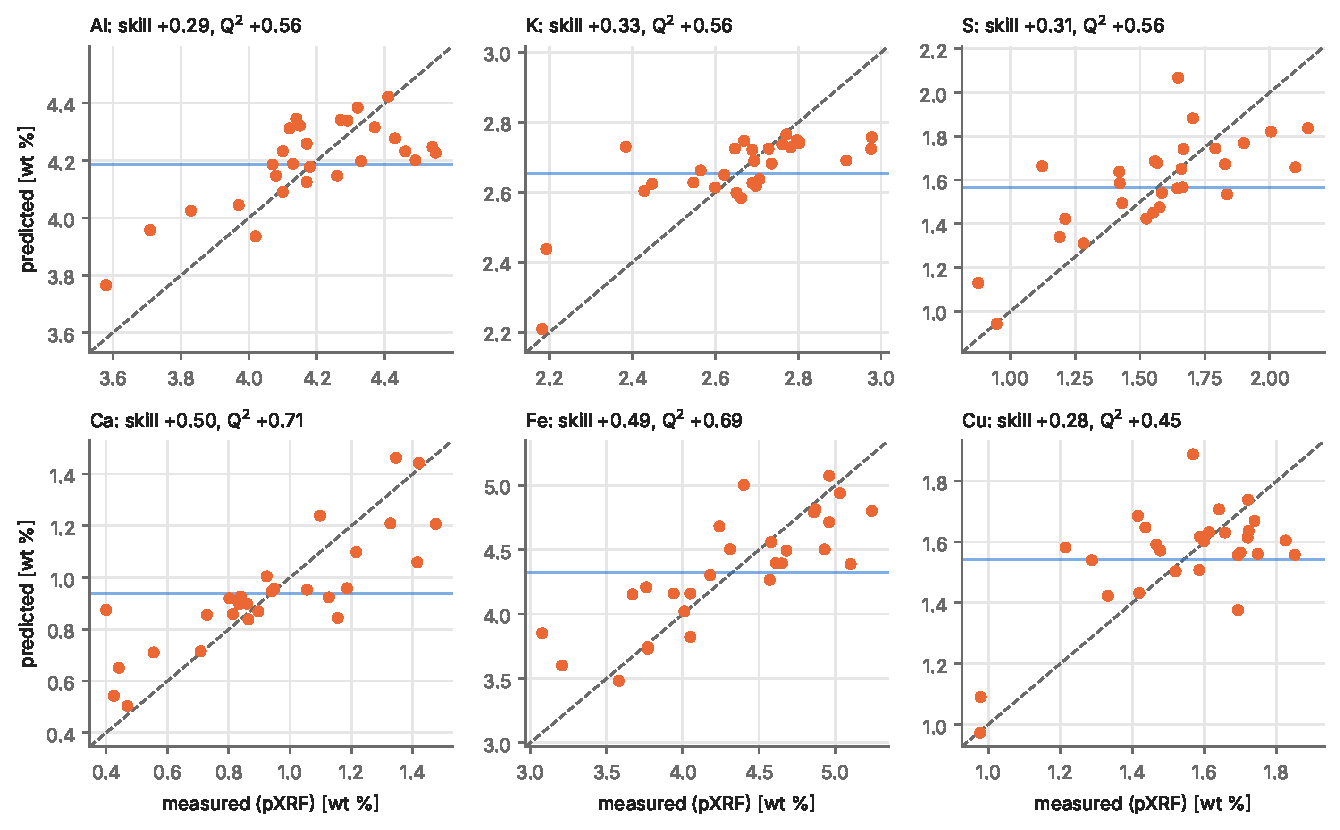
\includegraphics[width=0.9\linewidth]{pred_vs_meas.pdf}
  \caption{Predicted against measured composition (LOSO, PCA + ridge, crop means). Dashed: identity; blue: mean of
    the samples.}
  \label{fig:pred}
\end{figure}

\paragraph{More data per sample does not help.} Patch-level models see 40 times more rows, but they do not do
better than crop-level models (\cref{tab:benchmark}): the extra rows describe the variability within a sample,
which the label does not resolve. The HIDSAG-like cluster pipeline is not better than a single PLS. The 1D-CNN is
the weakest learned model: barely better than the mean predictor on crop means (skill +0.02) and +0.17 on patches,
where it has more rows to fit, still below PLS. With 28 independent labels, the bias of a linear model is a better
trade than the variance of a network.

\paragraph{Corrections that did not help.} \Cref{tab:robustness} tests whether the artefacts of \cref{sec:physics}
hurt the model. Removing the tray pixels from the crop means does not change the skill, nor does centring the
spectra per size fraction; the linear models already learn to ignore the grain-size direction when both fractions
are in the training set, and the centring removes some useful information. The fine fraction alone is more
informative than the coarse one, and using both is best.

\begin{table}[t]
  \centering\small
  \caption{Robustness checks (LOSO, mean skill over Al \ldots Cu and skill of three elements).}
  \label{tab:robustness}
  \begin{tabular}{llrrrrr}
\toprule
variant & model & samples & skill & Ca & Fe & Cu \\
\midrule
baseline & PCA + ridge (raw) & 28 & +0.29 & +0.51 & +0.49 & +0.28 \\
baseline & PLS (d1) & 28 & +0.24 & +0.48 & +0.39 & +0.30 \\
grain-size centring & PCA + ridge (raw) & 28 & +0.21 & +0.40 & +0.46 & +0.21 \\
grain-size centring & PLS (d1) & 28 & +0.18 & +0.42 & +0.39 & +0.32 \\
both fractions (25 samples) & PCA + ridge (raw) & 25 & +0.25 & +0.44 & +0.52 & +0.37 \\
both fractions (25 samples) & PLS (d1) & 25 & +0.22 & +0.56 & +0.38 & +0.35 \\
fine only (25 samples) & PCA + ridge (raw) & 25 & +0.18 & +0.09 & +0.48 & +0.45 \\
fine only (25 samples) & PLS (d1) & 25 & +0.19 & +0.50 & +0.18 & +0.31 \\
coarse only (25 samples) & PCA + ridge (raw) & 25 & +0.05 & +0.18 & +0.19 & +0.25 \\
coarse only (25 samples) & PLS (d1) & 25 & +0.12 & +0.51 & +0.35 & +0.32 \\
1000 px per crop & PCA + ridge (raw) & 28 & +0.28 & +0.49 & +0.51 & +0.27 \\
1000 px per crop & PLS (d1) & 28 & +0.22 & +0.47 & +0.40 & +0.30 \\
1000 px, tray masked & PCA + ridge (raw) & 28 & +0.26 & +0.46 & +0.50 & +0.28 \\
1000 px, tray masked & PLS (d1) & 28 & +0.23 & +0.49 & +0.39 & +0.25 \\
\bottomrule
\end{tabular}

\end{table}

% =====================================================================================================================
\section{Comparison with the reference benchmark}\label{sec:leakage}

The HIDSAG paper reports for GEOCHEM a mean absolute percentage error of \SI{0.021}{\percent} for Al and below
\SI{0.3}{\percent} for all nine major elements with the full spectral range, obtained with ``leave-one-out rounds''
of a clustering and regression pipeline \citep[Table 5]{Ehrenfeld2023}. \Cref{tab:mape} puts these numbers next to
ours. The mean predictor alone has a MAPE of \SI{4.5}{\percent} for Al; our best LOSO model reaches
\SI{3.1}{\percent}.

To find out which validation can produce the published numbers, \cref{tab:leakage,fig:leakage} evaluates the same
models with three splits of the patch-level data: random patches (80/20), leave one crop out, and leave one sample
out. Random patch splits put patches of every test sample in the training set; they inflate the skill and bring the
MAPE close to the SWIR-only column of the paper. No split brings it near the full-range column, which is two orders
of magnitude below the SWIR column of the same table. We conclude that the published GEOCHEM numbers were most
likely obtained with a split that shares samples between training and test, and that the full-range column in
addition contains an error of units or scale. They should not be used as a benchmark.

Under the same sample-wise protocol, the comparison is in favour of simpler models: our approximation of the
reference pipeline (cluster + PLS) reaches a skill of 0.22 on patches, a single PLS 0.26 and PCA + ridge on crop means
0.29 (\cref{tab:benchmark}). The approximation differs from the original in its details (the original uses a
probabilistic clustering, stochastic patch selection and ordinary least squares), so this ranking holds for our
re-implementation, not necessarily for the authors' code.

\begin{table}[t]
  \centering\small
  \caption{MAPE [\%] of the major elements: mean predictor and best model under LOSO, the HIDSAG-like pipeline under
    a random patch split, and the values reported by \citet[Table 5]{Ehrenfeld2023}.}
  \label{tab:mape}
  \begin{tabular}{lrrrrr}
\toprule
& \multicolumn{3}{c}{this work} & \multicolumn{2}{c}{HIDSAG paper} \\ \cmidrule(lr){2-4}\cmidrule(lr){5-6}
element & mean pred. & LOSO & random patches & SWIR & full \\
\midrule
Al & 4.5 & 3.1 & 2.7 & 2.5 & 0.021 \\
Si & 3.2 & 2.9 & 2.2 & 1.7 & 0.136 \\
P & 7.2 & 6.3 & 4.9 & 3.9 & 0.181 \\
S & 17.5 & 11.1 & 7.5 & 6.8 & 0.168 \\
K & 5.5 & 3.7 & 3.2 & 2.4 & 0.080 \\
Ca & 35.3 & 16.6 & 14.5 & 7.5 & 0.022 \\
Ti & 11.7 & 9.8 & 7.7 & 6.9 & 0.213 \\
Fe & 12.4 & 6.3 & 6.3 & 4.7 & 0.152 \\
Cu & 13.2 & 8.7 & 6.6 & 5.8 & 0.270 \\
\bottomrule
\end{tabular}

\end{table}

\begin{table}[t]
  \centering\small
  \caption{The same models under three splits of the patch-level data. Skill: mean over Al \ldots Cu.}
  \label{tab:leakage}
  \begin{tabular}{llrrrr}
\toprule
model & split & skill & \multicolumn{3}{c}{MAPE [\%]: Al, Ca, Cu} \\
\midrule
PLS & random patches (80/20) & +0.46 & 2.43 & 12.5 & 6.6 \\
PLS & leave one crop out & +0.38 & 2.78 & 13.6 & 7.6 \\
PLS & leave one sample out & +0.26 & 3.38 & 15.4 & 9.2 \\
cluster + PLS (HIDSAG-like) & random patches (80/20) & +0.43 & 2.70 & 14.5 & 6.6 \\
cluster + PLS (HIDSAG-like) & leave one crop out & +0.33 & 3.20 & 16.9 & 7.5 \\
cluster + PLS (HIDSAG-like) & leave one sample out & +0.22 & 3.79 & 19.1 & 8.6 \\
\bottomrule
\end{tabular}

\end{table}

\begin{figure}[t]
  \centering
  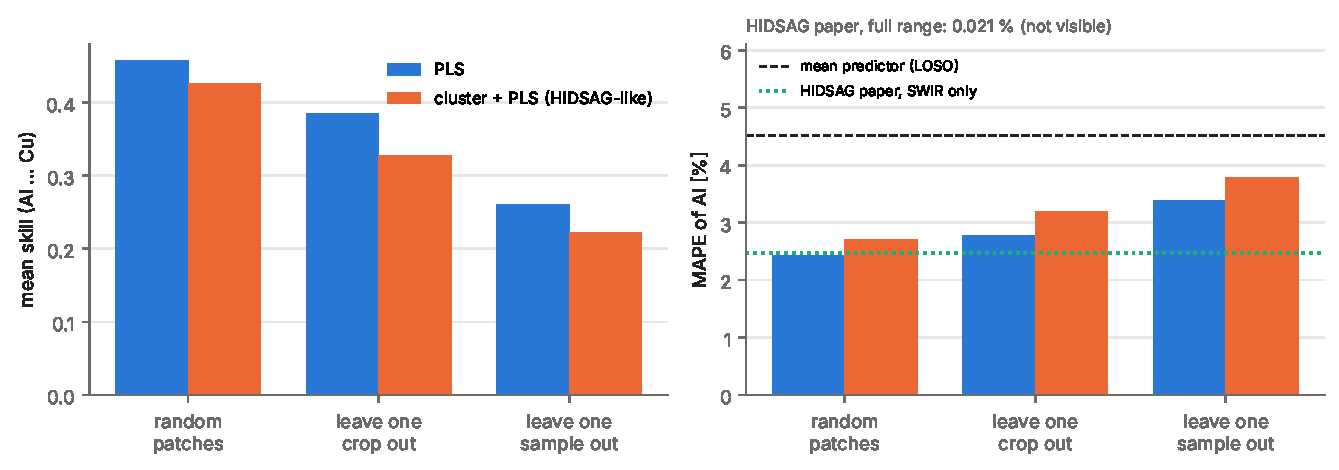
\includegraphics[width=0.9\linewidth]{leakage.pdf}
  \caption{Effect of the split on the measured accuracy. Left: mean skill. Right: MAPE of Al; dashed: mean
    predictor, dotted: value reported by the HIDSAG paper for the SWIR camera alone. Only the right-most pair measures the prediction of an unseen sample.}
  \label{fig:leakage}
\end{figure}

% =====================================================================================================================
\section{Main changes}\label{sec:lessons}

\Cref{tab:changes} lists the main modifications with respect to the original course notebook.

\begin{table}[H]
  \centering\small
  \caption{Main changes with respect to the original notebook.}
  \label{tab:changes}
  \begin{tabular}{p{0.2\linewidth}p{0.34\linewidth}p{0.36\linewidth}}
    \toprule
    & original notebook & this version \\
    \midrule
    Data used & one mean spectrum per sample (28 spectra) & all 106 crops, both size fractions, 1000 pixels per
      crop; patches of 25 pixels \\
    Spectral features & -- & VNIR binned to \SI{10}{nm}, noisy band edges removed;
      SNV, derivatives, continuum removal, band depths \\
    Validation & random split & leave one sample out, inner cross-validation grouped by sample, permutation test \\
    Reference & none & mean predictor; skill and $Q^2$ relative to it \\
    Models & 1D-CNN & PLS, PCA + ridge, cluster + PLS (reference pipeline), best band, 1D-CNN \\
    Interpretation & -- & absorption features, correlation spectra, pixel maps \\
    Artefacts & not examined & grain size, tray pixels, sensor striping quantified and tested \\
    Comparison with literature & published accuracy taken at face value & same models under leaky and honest
      splits \\
    Report & Jupyter notebook & this report, scripts for every table and figure, tests \\
    \bottomrule
  \end{tabular}
\end{table}

% =====================================================================================================================
\section{Further work and conclusions}\label{sec:next}

\paragraph{Conclusions.}
\begin{enumerate}
  \item Hyperspectral images of a sampled batch carry real but limited information about its chemistry. On samples
    not seen in training, the best model removes \SI{29}{\percent} of the error of the mean predictor on average,
    about half for Ca and Fe, about a third for K, S, Al and Cu, and little for Si, P and Ti. All skills are
    significant in a permutation test.
  \item The camera measures minerals. Elements are predictable when they reside in minerals with absorptions in
    the VNIR--SWIR range (Al and K in muscovite) or co-vary with them (Cu with alteration).
  \item With 28 labelled samples, regularised linear models are the right tools; a convolutional network and a
    clustering pipeline add variance, not skill. More pixels per sample do not compensate for few samples.
  \item Grain size changes the absorption depths more than composition does. Sample preparation should fix the
    size fraction, or the size distribution has to be measured alongside the spectra.
  \item The accuracy published for HIDSAG GEOCHEM is consistent with a validation that shares samples between
    training and test, and in part with an error of scale. It cannot serve as a target.
\end{enumerate}

\paragraph{Further work.} For the SAG mill, what matters is not the composition itself but hardness, grindability
and moisture. The HIDSAG subset GEOMET contains 146 drill-core samples with the Bond work index, copper and
molybdenum recoveries and other metallurgical tests, imaged with the same cameras. There, the reference pipeline was
validated on 21 samples held out from training \citep{Ehrenfeld2023}, i.e.\ by sample: its GEOMET results are a
legitimate baseline, and the natural starting point of the next phase, unlike its GEOCHEM results. Three lessons
carry over from this work: validate by sample (or by drill hole), report the skill with respect to the mean
predictor, and model the particle size. Whether the predicted composition should be an intermediate input to the
mill variables, or the spectra should be regressed on them directly, is an open question: the errors of this first
step would propagate into the second, which favours the direct route unless the composition adds information.

% =====================================================================================================================
\section*{Data and code}
HIDSAG is published under CC BY 4.0 \citep{HIDSAGdata}. All code, the derived crop spectra and the scripts for every
table and figure are available at \citet{Repo}.

\bibliographystyle{plainnat}
\bibliography{references}

\end{document}
